\section{Computador} 
Tendo em vista a metodologia de Project based learning – em que se incentiva a aprendizagem a partir da aplicação de conhecimentos e de habilidades através da experiência – esta pesquisa se propõe a construir um computador clássico (ilustrado a baixo), de forma que se possa por em prática a teoria estudada, possibilitando uma maior compreensão sobre a temática. Assim, o presente capítulo se debruça em detalhar o processo prático da construção do computador, sendo possível implementar as teorias, anteriormente vistas, na prática. Desta maneira, qualquer pessoa interessada, será capaz de construir seu próprio dispositivo, vivenciando o processo de Project based learning. 

\vspace{1cm}
\begin{figure}[H] \centering 
  \makebox[\textwidth][c]{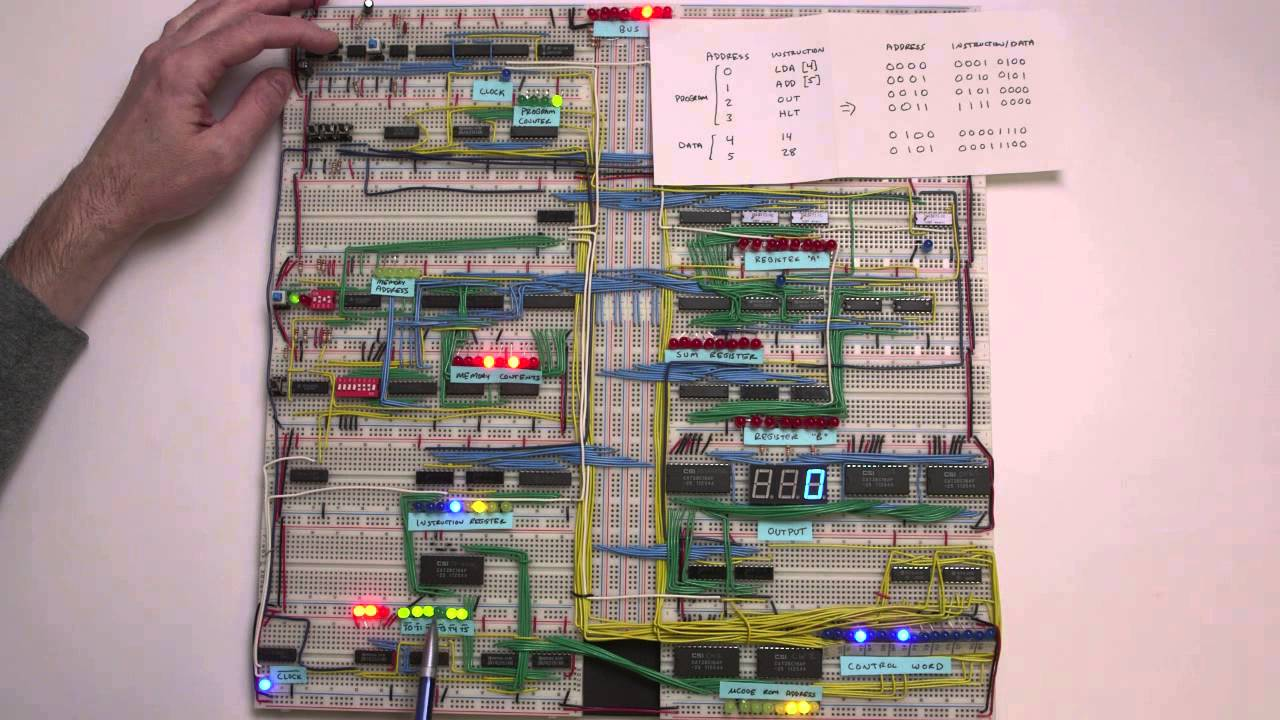
\includegraphics[width=0.8\textwidth]{breadboard_computer.jpg}}
  \caption{\label{breadboard_computer} Protótipo a ser implementado, imagem do site \href{https://eater.net/}{eater.net}} 
\end{figure}

Ainda, tem-se que a implementação física dos modelos contribuirá para academia, uma vez que os professores poderão usufruir dos mesmos como ferramentas didática, agregando para a compreensão da teoria ao aproximá-la da prática. 

No entanto, apesar desse capítulo ter sido reservado para descrever o passo a passo de como desenvolver um computador clássico apenas com portas lógicas simples, devido a alguns problemas esclarecidos na seção \ref{problems} não foi possível concluí-lo. Porém, de forma a manter a metodologia de Project based Learning, foi desenvolvido um sistema operacional que permitiu colocar em prática o conteúdo estudado ao implementar um processo de boot, usando o assembly intelx86. Além disso pode-se produzir um emulador de assembly, de forma didática e publicado na web,  a fim de contribuir com material para academia. Ademais, sugere-se que a proposta original seja adiada e implementada em um trabalho futuro. 

Apesar desta alteração no projeto, optou-se por compartilhar o conteúdo já produzido no início do processo de construção. 

\subsection{Módulos}
Para facilitar a compreensão e também o desenvolvimento do computador, este capítulo será dividido em alguns subcapítulos, cada qual abordando uma parte do computador.

\subsubsection{Clock}
O clock do computador é uma parte essencial para o seu funcionamento. Este tem a função de sincronizar todas as operações. A ação mais rápida que o computador consegue executar é equivalente a uma vibração do seu clock.

\subsubsection{Registers}
A maioria das CPUs possuem vários registradores que armazenam pequenas quantidades de dados processados pela CPU. Em nossa CPU de breadboard, criaremos três registradores de 8 bits: A, B e IR. Os registradores A e B são para uso geral. Já o IR (instruction register), apesar de funcionar da mesma forma, é usado para armazenar a instrução atual que está sendo executada.

\subsubsection{Arithmetic logic unit (ALU)}
A parte da unidade lógica aritmética (ALU) de uma CPU geralmente é capaz de executar várias operações aritméticas, bit a bit e de comparação em números binários. Em nossa CPU de breadboard, a ALU pode apenas adicionar e subtrair. Ele está conectado aos registradores A e B e gera a soma de A + B ou a diferença de A-B.

\subsubsection{Random access memory (RAM)}
A memória de acesso aleatório (RAM) armazena o programa que o computador está executando, bem como todos os dados que o programa precisa. Nosso computador de breadboard utiliza endereços de 4 bits, o que significa que ele terá apenas 16 bytes de RAM, limitando o tamanho e a complexidade dos programas que poderá executar.

\subsubsection{Program counter}
O contador do programa (Program counter) conta em binário para acompanhar a instrução que o computador está executando no momento.

\subsubsection{Output register}
O registrador de saída é semelhante a qualquer outro registrador (como os registradores A e B), exceto que, em vez de exibir seu conteúdo em binário em 8 LEDs, ele exibe seu conteúdo de forma decimal em um display de 7 segmentos, o que requer uma lógica complexa.

\subsubsection{CPU control logic}
A lógica de controle é o coração da CPU, é o que define os códigos de operação (opcode) que o processador reconhece e o que acontece quando ele executa cada instrução.

\newpage


